\chapter{力}

    现在我们开始学习力学知识.力学所要解决的中心课题
是力和物体运动的关系.这一章学习有关力的知识,下一章
学习怎样描述物体的运动.有了这两章的知识淮备,到第三
章就可以学习力和物体运动的关系了.

    在这一章里,我们要在复习初中所学知识的墓础上,进一
步学习力的知识,以加深和扩大我们对力的理解.研究力学
问题常常要分析物体的受力情况.这一章里要介绍怎样分析
物体的受力情况,希望同学们初步学会分析方法,并在以后的
学习中逐步熟悉它,掌握它.最后,我们还要在学习力的合成
与分解的基础上,学习矢量的概念和矢量运算的特殊性.


\section{力}
    人们对力的认识,最初是从日常生活和生产劳动中得到
的,是和人力相联系的.用手推动小车,提起重物,拉长或压
缩弹簧,肌肉会感到紧张,我们就说,人对小车、重物、弹簧用
了力,后来人们把力的概念加以扩展,把凡是能和人力起相
同效果的作用都叫做力.机车牵引列车前进,机车对列车施
加了力.汽锤锻打工件,汽锤对工件施加了力.这样,人们建
立了这样的认识:\textit{力是物体对物体的作用}.

一个物体受到力的作用,一定有另一个物体施加这种作
用.前者是受力物体,后者是施力物体,只要有力发生,就一
定有受力物体和施力物体.有时为了方便,只说物体受到了
力,而没有指明施力物体,但施力物体一定是存在的.

    力是有大小的.我们在初中学过,力的大小可以用测力
计来测量.在国际单位制中力的单位是\textbf{牛顿},简称牛,国际符
号是N,日常生活和生产中常用的力的单位是千克力,牛顿
和千克力的关系是:1千克力$=9.8$牛.

    力不但有大小,而且有方向.物体受到的重力是竖直向
下的,物体在液体中受到的浮力是竖直向上的,力的方向不
同,它的作用效果也不同.用力拉弹簧,弹簧就伸长;用反方
向的力压弹簧,弹簧就缩短.
作用在运动物体上的力,如果方
向与运动方向相同,将加快物体的运动;如果方向与运动方向
相反,将阻碍物体的运动.可见,要把一个力完全表达出来,
除了说明力的大小外,还要指明力的方向.

为了直观地说明力的作用,常常用一根带箭头的线
段来表示力.线段是按一定比
例(标度)画出的,它的长短表
示力的大小,它的指向表示力
的方向,箭头或箭尾表示力的
作用点,箭头所沿的直线叫做
力的作用线.这种表示力的方
头,叫做\textbf{力的图示}.图1.1中表示的是作用在小车上的100牛
的力.

\begin{figure}[htp]\centering
\begin{tikzpicture}[>=stealth, thick]

\draw (0,0)--(2,0)--(2,1)--(0,1)--(0,0);

\fill [pattern = north east lines] (-1,-.75) rectangle (3,-.5);
\draw(-1,-.5)--(3,-.5);
\draw (.5,-.25) circle (.225);
\draw (1.5,-.25) circle (.225);
\draw (.5,-.25) circle (.1);
\draw (1.5,-.25) circle (.1);

\draw[->, dashed](3,0.5)--(-2,0.5);
\draw[very thick](0,.5)--(-2,0.5);
\foreach \i in {-.4,-.8,-1.2,-1.6,-2}
{
    \draw (\i,0.6)--(\i,.5);
}

\draw (-1,1)--(-1,1.1);
\draw (-0.6,1)--(-0.6,1.1);

\draw[-] (-1,1)--(-0.6,1);
\node at (-0.8,1.35){\small 20牛顿};


\end{tikzpicture}
\caption{图中的虚线表示力的作用线}
\end{figure}

我们从初中开始学习物理以来,见过的力的名称已经相当多了.各种力可以用不同的方法来分类.
一种是根据力的性质来分类的,如重力、弹力、摩擦力、分子力、电磁力等
;另一种是根据力的效果来分类的,如拉力、压力、支持力、
动力、阻力等等.拉力、压力、支持力实际上都是弹力,只是效
果不同.不论是什么性质的力,只要效果是加快物体的运动,
就可以叫它为动力;效果是阻碍物体的运动,就可以叫它为阻
力.今后我们还会遇到根据效果来命名的力的名称.

    从力的性质来看,力学中经常遇到的有重力、弹力、摩擦
力.下面几节就分别介绍这三种力.


\section{重力}
    地球上一切物体都受到地球的吸引作用.这种由于地球
的吸引而使物体受到的力叫做\textbf{重力}.重力也常常叫做\textbf{重量}.

    重力不但有大小,而且有方向.悬挂物体的绳子,静止时
总是竖直下垂的.自由落向地面的物体,总是竖直下落的,可
见重力的方向是竖直向下的.物体所受的重力的大小跟物体
的质量成正比,质量越大,所受的重力越大.1千克质量的物
体所受的重力是1千克力,即9.8牛;2千克质量的物体所受
的重力是2千克力,即$2\times 9.8$牛等等,把物体挂在绳子上,
物体静止时拉紧悬绳的力,大小等于物体所受的重力.把物
体放在静止的水平支持物上,物体压在水平支持物上的力,大
小也等于物体所受的重力.

    一个物体的各部分都要受到地球对它的作用力,我们可
以认为重力的作用集中于一点,这一点叫做物体的\textbf{重心}.如
图1.2那样用手指支持一根铅
笔,我们可以找到一个位置,使
铅笔水平地支持在手指上,手
指上方铅笔上的$C$点就是铅笔
的重心.这时铅笔受到两个力:
竖直向上的手指的支持力$N$,
竖直向下的重力$G$.这两个力大小相等方向相反,而且作用
在同一直线上,从初中学过的二力平衡条件知道,这时铅笔保
持平衡.如果重心$C$不在手指的正上方,支持力$N$和重力$G$,
将不在同一直线上,铅笔就不能保持平衡了.
\begin{figure}[htp]
\centering
\includegraphics[scale=.5]{fig/1-2.PNG}
\caption{}
\end{figure}

    质量均匀分布的物体(均匀物体),重心的位置只跟物体
的形状有关.有规则形状的均匀物体,它的重心就在几何中
心上.例如,均匀直棒的重心在棒的中点,均匀球体的重心在
球心,均匀圆柱体的重心在轴线的中点(图1.3).

 \begin{figure}[htp]\centering
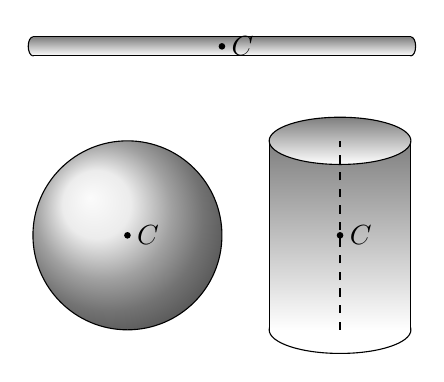
\begin{tikzpicture}[scale=.6]
\draw [shade] (0-5,6) ellipse [x radius=.1, y radius=.2];
\draw[shade] (6-3,6) ellipse [x radius=.1, y radius=.2];
\shade (0-5,6-.2) rectangle (6-3,6+.2);
\draw (0-5,6.2)--(6-3,6.2);
\draw (0-5,5.8)--(6-3,5.8);
\node at (-1,6) [right] {$C$};
\fill (-1,6) circle(2pt);


\draw (1.5,0) ellipse [x radius=1.5, y radius=.5];
\shade (0,0) rectangle (3,4);
\shade (1.5,4)[draw] ellipse [x radius=1.5, y radius=.5];
\draw (0,0)--(0,4);
\draw (3,0)--(3,4);

\draw [dashed](1.5,0)--node [right] {$C$}(1.5,4);
\fill (1.5,2) circle(2pt);

\shade [draw, ball color =gray!20] (-3,2)node [right] {$C$} circle(2);
\fill (-3,2) circle(2pt);
\end{tikzpicture}
\caption{}
 \end{figure}

    不均匀物体的重心的位置,除跟物体的形状有关外,还跟
物体内质量的分布有关.载重汽车的重心随着装货多少而不
同,起重机的重心随着提升重物的重量和高度而变化.

    用简单的实验方法可以求出形状不规则成者质量不均匀
的薄板状物体的重心.如图1.4所示,先在$A$点把物体悬挂
起来,当物体处于平衡时,它所受的重力跟悬绳的位力在同一
直线上,也就是说,重心一定在通过$A$点的竖直线$AB$上.然
后,在$D$点把物体悬挂起来,同样可以知道,重心一定在通过
$D$点的竖直线$DE$上.$AB$和$DE$的交点$C$就是物体的重心.


\begin{figure}[htp]
\centering
\includegraphics[scale=1.3]{fig/1-4.pdf}
\caption{}
\end{figure}

\section{弹力}
被拉长或压缩的弹簧对跟它接触的小车发生力的作用,
可以使小车运动起来(图1.5).被弯曲的细木棍或细竹竿对
跟它接触的圆木发生力的作用,可以把圆木推开(图1.6).
物体的伸长、缩短、弯曲等等,总之物体的形状或体积的改变,叫
做形变.上面的例子说明,发生形变的物体,由于要恢复原
状,对跟它接触的物体会产生力的作用,这种力叫做\textbf{弹力}.

\begin{figure}[htp]\centering
\begin{tikzpicture}[>=stealth, thick]
\tikzstyle{spring}=[thick,decorate,decoration={aspect=0.5, segment length=2mm, amplitude=2mm,coil}]

\draw [->](0.5,1.2)--(1.5,1.2);
\draw (0,0) rectangle (2,.25);
\draw (.75,.25) rectangle (1.25,1);

\fill [pattern = north east lines] (-1,-.75) rectangle (3,-.5);

\fill [pattern = north east lines] (4,-.5) rectangle (4.2,1);
\draw (4,-.5)--(4,1);

\draw(-1,-.5)--(3,-.5);
\draw (.5,-.25) circle (.225);
\draw (1.5,-.25) circle (.225);
\draw (.5,-.25) circle (.1);
\draw (1.5,-.25) circle (.1);

\draw [spring](2,.12)--(4,.12);

\node at (1,-1.5){甲:被拉长的弹簧使小车向右运动};
\end{tikzpicture}
\begin{tikzpicture}[>=stealth, thick]
\tikzstyle{spring}=[thick,decorate,decoration={aspect=0.5, segment length=1.5mm, amplitude=2mm,coil}]
\draw [<-](0.5,1.2)--(1.5,1.2);
\draw (0,0) rectangle (2,.25);
\draw (.75,.25) rectangle (1.25,1);

\fill [pattern = north east lines] (-1,-.75) rectangle (3,-.5);

\fill [pattern = north east lines] (3.5,-.5) rectangle (3.7,1);
\draw (3.5,-.5)--(3.5,1);

\draw(-1,-.5)--(3,-.5);
\draw (.5,-.25) circle (.225);
\draw (1.5,-.25) circle (.225);
\draw (.5,-.25) circle (.1);
\draw (1.5,-.25) circle (.1);

\draw [spring](2,.12)--(3.5,.12);

\node at (1,-1.5){乙:被压缩的弹簧使小车向左运动};

\end{tikzpicture}
\caption{}

\end{figure}

\begin{figure}[htp]
\centering
\includegraphics[scale=.5]{fig/1-6.PNG}
\caption{被弯曲的细木棍把圆木推开}
\end{figure}

    地球对物体产生重力,并不需要地球和物体直接接触.弹
力则不同,它只有在物体直接接触并产生形变的时候才能产
生,把一本书放在泡沫塑料上(图1.7),书把泡沫塑料压弯,
被压弯的泡沫塑料要恢复原状,产生向上的弹力,这就是它对
书的支持力.把一个物体挂在弹簧上,物体把弹簧拉长,被
拉长的弹簧要恢复原状,产生向上的弹力,这就是它对物体的
拉力.
\begin{figure}[htp]
\centering
\includegraphics[scale=.5]{fig/1-7.PNG}
\caption{}
\end{figure}

    不仅泡沫塑料、弹簧等能够发生形变,任何物体都能够发
生形变,不能发生形变的物体是不存在的.不过有的形变比
较明显,直接可以看得见;有的形变极其微小,要用仪器才能
显示出来.把书放在桌面上,书压桌面,使桌面和书都发生极
其微小的形变.发生形变的书要恢复原状,对桌面产生向下
的弹力,这就是书对桌面的压力.发生形变的桌面要恢复原
状,产生向上的弹力,这就是桌面对书的支持力.\textit{凡是支持物体对物体的支持力,
都是支持物因为发生形变而对物体产生弹力;支持力的方向总是垂直于支持面并指向
被支持的物体}(图1.8).
把电灯挂在电线上,电灯拉紧电线,使电灯和电线
都发生极其微小的形变,发生形变的电灯要恢复原状,对电
线产生向下的弹力,这就是电灯对电线的拉力.发生形变的
电线要恢复原状,产生向上的弹力,这就是电线对电灯的拉
力.\textit{凡是一根线(或绳)对物体的拉力,都是这根线(或绳)因
为发生形变而对物体产生的弹力;拉力的方向总是指向线收
缩的方向}(图1.9).

\begin{figure}[htp]\centering
\begin{tikzpicture}[>=stealth, thick]


\draw [fill=black!20](0,0) rectangle (1.5,.75);
\fill [pattern = north east lines] (-1,-.25) rectangle (3,0);
\draw(-1,0)--(3,0);
\draw[->](.75,.375)--(.75,1.5);
\node at (.75,1.75){$N$};
\fill (.75,.375) circle[radius=1.5pt];
\node at (1,-.75){甲};

\end{tikzpicture}\qquad \qquad 
\begin{tikzpicture}[>=stealth, thick]


\draw [rotate=30, fill=black!20] (0,0) rectangle (1.5,.75);
\fill [rotate=30, pattern = north east lines] (-1,-.25) rectangle (3,0);
\draw[rotate=30] (-1,0)--(3,0);
\fill[rotate=30] (.75,.375) circle[radius=1.5pt];
\draw[rotate=30, ->](.75,.375)--(.75,1.5);
\node at (.25,1.75){$N$};
\draw(-.85,-.5)--(3,-.5);

\node at (1,-1){乙};

\end{tikzpicture}

\caption{支持力的方向}



\end{figure}

\begin{figure}[htp]\centering
\begin{tikzpicture}[>=stealth, thick]

\fill [pattern = north east lines] (0,0) rectangle (1,.25);

\draw(0,0)--(1,0);
\draw(.5,0)--(.5,-3);
\draw [fill=black!50] (.5,-3.25) circle (.225);

\draw[->](.5,-3)--(.5,-2);
\node at (.75,-2){$F$};
\node at (.5,-4){甲};

\end{tikzpicture}\qquad \qquad
\begin{tikzpicture}[>=stealth, thick]
\fill [pattern = north east lines] (-2,0) rectangle (-1,.25);
\fill [pattern = north east lines] (1,0) rectangle (2,.25);
\draw(-2,0)--(-1,0);  \draw(2,0)--(1,0);
\draw (-1.5,0)--(0,-3);  \draw(1.5,0)--(0,-3);
\draw[->] (0,-3)--(-.75,-1.5);  \draw[->] (0,-3)--(0.75,-1.5);
\draw [fill=black!30] (-.3,-3.5) rectangle (.3,-3);
\node at (0,-4){乙};
\node at (-1,-2){$F_1$};\node at (1,-2){$F_2$};

\end{tikzpicture}

\caption{线的拉力的方向}



\end{figure}

\section*{阅读材料:显示微小形变的装置}

图1.10是一种显示微小形变的装置,它可以把微小形变
“放大”到可以直接看出来.在一张大案子上放两个平面镜$M$
和$N$,让一束光线依次被这两面镜子反射,最后射到一个刻
度尺上,形成一个光点,只要用力压桌面,镜子就要向箭头所
示的方向倾斜. 由于两面镜子之间的距离较大,光点就会在
刻度尺上有明显的移动,而把桌面的形变显示出来.

    这个实验井不难做,希望同学们在教师指导下做一做,用
手压一下桌面,或者在桌面上放一个物体,看看光点是否发生
明显的移动.这个实验可以使你看到放在桌面上的一本书确
实会使桌面发生形变.

    在物理学实验中常常需要把微小的效应“放大”而显示出
来,在今后的学习中,希望同学们注意这一类实验的设计.

\begin{figure}[htp]
\centering
\includegraphics[scale=1.3]{fig/1-10.pdf}
\caption{显示微小形变的装置
}
\end{figure}

\subsection*{练习一}
\begin{enumerate}
\item  举出几个实例来说明力是物体对物体的作用.
\item 放在水平面上的物体(图1.8甲)受到几个力的作用?
  各是什么物体对它的作用,是哪种力?画出物体受力的示意
  图.
\item 用一根绳子把小球挂在天花板上(图1.9甲),小球受
  到几个力的作用?各是什么物体对它的作用,是哪种力?画出
  小球受力的示意图.
\item 用两根绳子把物体挂在天花板上(图1.9乙),这个物
  体受到几个力的作用?各是什么物体对它的作用,是哪种力?
  画出物体受力的示意图.
 \item 找一个薄板状的物体,用书中所讲的悬挂方法求出
  这个物体的重心.
 \item 放在水平桌面上的两个小球,它们靠在一起但不互
相挤压,它们之间有弹力作用吗?为什么?
\item 用下面的简单装置也可以显示微小形变.找一个大
玻璃瓶,装满水,塞上中间插有细管的瓶塞.用手按压玻璃瓶,
细管中的水面就上升;松开手,水面又降回原处.这说明玻璃瓶
遇到按压时发生弹性形变.实际做一下这个实验.
\end{enumerate}

\section{胡克定律}
力的大小跟形变的大小有关系,形变越大,弹力也越
大;形变消失,弹力就随着消失.对于拉伸(或压缩)形变来说,
伸长(或缩短)的长度越大,产生的弹力就越大,弹簧伸长或
缩短的长度越大,弹力就越大,这是我们从经验中都知道的.
把一个物体挂在悬线上,物体越重,把悬线拉得越长(实际上
还是看不出来),悬线的拉力也越大,物体发生弯曲时产生的
形变叫做弯曲形变.对于弯曲形变来说,弯曲得越厉害,产生
的弹力就越大.把弓拉得越满,箭就射出得越远,把一个物
体放在支持物上,物体越重,支持物弯曲得越厉害,支持力就
越大.还有一种叫做扭转形变,在金属丝的下面挂一个横
杆,用力扭这个横杆,金属丝就发生扭转形变(图1.11).放
开手,发生扭转形变的金属丝产生的弹力会把横杆扭回来.金
属丝的扭转角度越大,弹力就越大.

\begin{figure}[htp]\centering
\begin{tikzpicture}[>=stealth, thick]

\fill [pattern = north east lines] (0,0) rectangle (1,.25);

\draw(0,0)--(1,0);

\draw(.5,-3)--(.5,0);
\draw[double, thick, gray](-1,-4)--(2,-2);
\draw [->](-1,-4) arc [start angle=180, end angle=170, radius=4.5];
\draw [->](2,-2) arc [start angle=0, end angle=-10, radius=4.5];

\node at (.5,-5){甲};

\end{tikzpicture}
\qquad 
\begin{tikzpicture}

\fill [pattern = north east lines] (0,0) rectangle (1,.25);

\draw(0,0)--(1,0);
\draw (.2,-4) rectangle (.75,0);

\draw(.4,0)--(.4,-3.5);
\draw(.55,0)--(.55,-3.5);


\node at (.5,-5){乙};
\end{tikzpicture}
\qquad 
\begin{tikzpicture}[>=stealth]

\fill [pattern = north east lines] (0,0) rectangle (1,.25);

\draw(0,0)--(1,0);

\draw (.2,-4) rectangle (.75,0);

\draw[dashed](.4,0)--(.4,-3.5);
\draw[dashed](.55,0)--(.55,-3.5);

\draw(.4,0)--(.3,-3.5/2);
\draw(.55,0)--(.35,-3.5);

\node at (.5,-2.75){$\theta$};
\node at (.5,-5){丙};

\draw [->](.55,-2.5) arc [start angle=270, end angle=267, radius=3];

\end{tikzpicture}



\caption{甲图表示用扭横杆的办法使金属丝发生扭
转形变.乙图是放大了的未发生扭转形变
的金属丝的示意图.丙图是放大了的发生
扭转形变的金属丝的示意图,$\theta$角可以用
来表示扭转形变的大小}
\end{figure}



    定量地研究各种形变中弹力和形变的关系比较复杂,我
们经常遇到的是弹簧的拉伸(或压缩)形变.实验表明:\textit{弹簧
弹力的大小$f$和弹簧伸长(或缩短)的长度$x$成正比.}
写成公式就是
\[f=kx\]
其中$k$是比例常数,叫做弹簧的\textbf{倔强系数}.倔强系数是一个
有单位的量.在国际单位制中,$f$的单位是牛,$x$的单位是
米,$k$的单位是牛/米.倔强系数在数值上等于弹簧伸长(或
缩短)单位长度时的弹力.倔强系数跟弹簧的长度、弹簧的材
料、弹簧丝的粗细等等都有关系.弹簧丝粗的硬弹簧比弹簧
丝细的软弹簧倔强系数大.对于直杆和线的拉伸(或压缩)形
变,也有上述正比关系,这个规律是英国科学家胡克发现的,
叫做\textbf{胡克定律}.

    胡克定律有它的适用范围.物体的形变过大,超出一定
限度,上述正比关系将不再适用,这时即使撤去外力,物体也
不能完全恢复原状.这个限度叫做\textbf{弹性限度}.胡克定律在弹
性限度内适用.弹性限度内的形变叫做\textbf{弹性形变}.本书中提
到的形变,除非特别指明,一般是指弹性形变.

\subsection*{练习二}
\begin{enumerate}
\item 把一个重量为2牛的物体挂在弹簧上,物体静止时受
到的弹簧的弹力有多大?为什么?
\item 把重量相同的两个物体分别挂在两根不同的弹簧
上,一根弹簧伸长的长度小,另一根伸长的长度大,哪根弹簧
的倔强系数大?
\item 一根弹簧的倔强系数是100牛/米,伸长的长度为2厘
米时,弹簧的弹力有多大?另一根弹簧的倔强系数是2000
牛/米,缩短的长度为3厘米时,弹簧的弹力有多大?
\item 一根弹簧,不挂物体时长15厘米,挂上0.5千克的物
体时长18厘米.这根弹簧的倔强系数有多大?
\end{enumerate}

\section{摩擦力}
    摩擦力也是发生在两个互相接触的物体之间.当一个物
体在另一个物体表面上做相对滑动的时候,要受到另一个物
体阻碍它运动的力,这种力叫做滑动摩擦力.滑动摩擦力的
方向总跟接触面相切,并且跟物体的相对运动的方向相反(图
1.12).实验表明:\textit{滑动摩擦力跟压力成正比
也就是跟一个物体对另一个物休表面的垂直作用力成正比.}
用$f$表示滑动摩擦力的大小,用$N$表示压力的大小,那么
\[f=\mu N,\]
\begin{figure}[htp]\centering
\begin{tikzpicture}[>=stealth, thick]
\fill [fill=black!30, draw] (2,0.35) rectangle (3.5,1.25);


\fill [pattern = north east lines] (0,0) rectangle (5,.25);
\draw (0,.25)--(5,.25);

\draw[->] (2,0.35)--(1,0.35);
\node at (0.75,0.35){$f$};
\draw[->] (4,0.75)--(5,0.75);
\node at (6,1.2){物体$A$的运动方向};
\node at (5.5/2,1.6/2){$A$};
\node at (5.5/2,-.25){$B$};
\end{tikzpicture}
\caption{滑动摩擦力$f$的方向.为了清楚地表示摩
擦力,此图把相互接触的两个物体画得隔
开一些.
}
\end{figure}
其中$\mu$是比例常数,叫做\textbf{滑动摩擦系数}.滑动摩擦系数是由
制成物体的材料决定的,材料不同,两物体间的滑动摩擦系数
也不同.滑动摩擦系数还跟接触面的粗糙程度有关.在相同
的压力下,滑动摩擦系数越大,滑动摩擦力就越大.滑动摩擦
系数是两个力的比值,没有单位.表1.1列出了在通常情况下
几种材料间的滑动摩擦系数.

\begin{table}[htp]\centering
\caption{几种材料间的滑动摩擦系数}
\begin{tabular}{cc}
\hline
材料   &  滑动摩擦系数\\
\hline
钢—钢     & 0.25 \\
木—木   & 0.30 \\
木—金属   &  0.20\\
皮革—铸铁   &  0.28\\
钢—冰   &  0.02\\
木头—冰   &  0.03\\
橡皮轮胎—路面(干)   &  0.71\\
\hline
\end{tabular}
\end{table}

    除了滑动摩擦,还有滚动摩擦.滚动摩擦是一个物体在
另一个物体表面上滚动时产生的摩擦.滚动摩擦比滑动摩擦
小得多,滚动轴承就是利用滚动摩擦小的事实制成的.

    滑动摩擦和滚动摩擦都是一个物体在另一个物体表面上
有相对运动的时候发生的.那么,互相接触的两个物体处于
相对静止的时候,是不是也可以发生摩擦呢?我们用不大的力
来推桌子,虽然桌子应该沿着力的方向运功,有相对于地板运
动的趋势,但并没有把桌子推动,就是因为桌腿跟地板之间发
生了摩擦.这个摩擦力和推力都作用在桌子上,它们的大小
相等,方向相反,彼此平衡,因此桌子保持不动.这时所发生
的摩擦叫静摩擦,静摩擦力的方向总跟接触面相切,并且跟
物体相对运动趋势的方向相反.

    逐渐增大对桌子的推力,如果推力还不够大,桌子仍旧保
持不动,静摩擦力跟推力仍旧彼此平衡.可见静摩擦力随着
推力的增大而增大.但是静摩擦的增大有一个限度,静摩擦
力的最大值叫最大静摩擦力.推力超过最大静摩擦力,就可
以把桌子推动了.最大静摩擦力等于使桌子开始运动所需的
最小推力.


\section*{阅读材料:力的种类}
    在力学中经常遇到的有重力、弹力和摩擦力,以后在热学
中要遇到分子力,在电学中要遇到电磁力.在课文中我们曾
经提到,重力、弹力、摩擦力、分子力、电磁力等是根据力的性
质来分类的,即认为它们是属于不同性质的力,其实这种认
识只是反映了人们对力的认识的一个阶段.随着科学的发展,
人们对力的探索已经从宏观物体进入到原子、分子的微观领
域,因而对力的一认识也进一步深化了.现代科学研究告诉我
们,通常见到的重力、弹力、摩擦力、分子力、电磁力等都可以
归结为两种基本的相互作用,即万有引力和电磁力.

    关于万有引力,我们将在第五章学习.万有引力是由于物
体具有质量而在物体之间产生的一种相互作用.这种力普遍
存在于宇宙万物之间.在宇宙天体之间,在宏观物体之间,在
原子、分子等粒子之间,都存在着这种相互作用.两个通常物体
之间的万有引力极其微小,我们觉察不到它,可以不予考虑.但
是,在天体系统中万有引力却起着决定性的作用.在天体中质
量还算很小的地球对其他物体的万有引力已经具有巨大影
响,它把人类、大气和所有地面物体束缚在地球上,它使月球
和人造地球卫星绕地球旋转而不能离去.重力就是地面附近
的物体由于受到地球的万有引力而产生的.太阳系中的八大
行星绕太阳旋转而不离去,是由于万有引力的作用.银河系里
的球状星团——由上百万个恒星聚在一起并呈球状的恒星集
合体——聚集不散,也是由于万有引力的作用.

    电磁力是存在于电荷之间的一种相互作用.静止电荷之
间有电力,运动电荷之间除了电力外还有磁力.电力和磁力
是有联系的,常常总称为电磁力.我们知道,原子是由带正电
的原子核和绕核旋转的带负电的电子组成的,分子是由原子
组成的.原子或分子本身能够形成,是由于电磁力的作用.分
子之间的电磁力就构成了我们通常所说的分子力.我们所看
到的多种多样的宏观物体是由原子或分子组成的,它们能聚
集不散而且使物体构成一定的形态,就是由于原子或分子之
间的电磁相互作用.从微小的原子到通常的物体,正是电磁
力把物质结合在一起的.

    当我们便物体发生形变的时侯,物体中原子或分子之间
的距离发生改变,原子或分子之间的电磁力要反抗物体发生
形变,这就形成了我们通常所说的弹力.摩擦力也可以归结
为电磁力.虽然从原子或分子之间的电磁力来完满地解释摩
擦力很为复杂,至今还没有一种很好的理论,但是大家公认摩擦
力说到底也还是电磁力的一种表现.

    我们看到,从宇宙天体到微小的原子,这中间只有两种基
本的相互作用:万有引力和电磁力.现代科学研究又深入一
步,深入到原子核内部,深入到研究质子、中子等粒子的相互
作用.人们在这个领域又发现了两种基本的相互作用,分别
叫做强相互作用和弱相互作用.这两种相互作用这里不再介绍了.

    这样,人类认识到在自然界中只存在四种基本的相互作
用:万有引力,电磁力,强相互作用,弱相互作用.小到比原
子还小的粒子,大到宇宙天体,其间表现出很不相同的多种多
样的相互作用,都可以用少数几种基本的相互作用来说明,这
是物理学的巨大胜利.然而人类的认识是没有止境的,今天
认为基本的相互作用只有四种,明天会不会统一成更少的几
种甚至一种相互作用呢?大物理学家、相对论的创立者爱因斯
坦(1879—1955),晚年致力于这方面的工作,企图把万有引力
和电磁力统一起来.现在有不少物理学家致力于这方面的研
究,企图把四种相互作用统一起来,并且取得了进展.这是物
理学的前沿阵地,物理学好象一座正在施工中的大厦,它己
经建筑得很壮观了,但还没有竣工,看来永远也不会竣工,更
壮观的还在后面.现在的青年学生,将来就可能成为修建这
座大厦的建筑师.

\subsection*{练习三}
\begin{enumerate}
\item  在东北的冬季伐木工作中,许多伐下的木料被装在
雪橇上,用马拉着在冰道上运出去.一个有钢制滑板的雪橇,
上面装着木料,共重$4.9\times 10^4$牛.在水平的冰道上,马要在水平
方向用多大的力才能够拉着雪橇匀速前进?

\item  用20牛的水平的力拉着一块重量是40牛的砖,可以
使砖在水平地面上匀速滑动.求砖和地面之间的滑动摩擦系
数.
\item  要使重量是400牛的桌子从原地移动,必须最小用
200牛的水平推力.桌子从原地移动以后,为了使它继续做匀
速运动,只要160牛的水平推力就行了.求最大静摩擦力和滑
动摩擦系数.如果用100牛的水平推力推桌子,这时静摩擦力
有多大?

\item  做下面的实验:用一根橡皮绳把书吊起来,当书静
止不动的时候,测出橡皮绳伸长的长度.把书放在桌子上,水
平拉橡皮绳,使书做匀速运动,再测出橡皮绳伸长的长度.设
橡皮绳伸长的长度跟外力成正比,根据测出的数据粗略地算
出书和桌面之间的滑动摩擦系数.
\end{enumerate}


\section{牛顿第三定律}
我们知道,力是物体对物体的作用,只要有力发生,就一
定要有受力物体和施力物体.施力物体是不是也要受到受力
物体给予它的力呢?力是物体间的单方面作用,还是物体间
的相互作用?

    用手拉弹簧,手的肌肉发生紧张(形变),同时弹簧也发生
形变,这时不但弹簧受到手的拉力,手也受到弹簧的拉力.坐
在椅子上用力推桌子,会感到桌子也在推我们,我们的身体要
向后移.在平静的水面上,在一只船上用力推另一只船,另一
只船也要推前一只船,两只船将同时向相反方向运动(图1.13).在水面上放两个软木塞,一个软木塞上放一个小磁铁,
另一个软木塞上放一个小铁条(图1.14),可以看到,由于小
磁铁和小铁条相互吸引,两个软木塞相向运动起来.地球和
地面上物体之间的作用也是相互的,地面上的物体受到地球
的吸引,即受到重力,地球也受到地面上的物体的吸引.

\begin{figure}[htp]\centering
\includegraphics[scale=.5]{fig/1-13.png}
\caption{}
\end{figure}

\begin{figure}[htp]\centering
\includegraphics[scale=.7]{fig/1-14.png}
\caption{}
\end{figure}

观察和实验表明,两个物体之间的作用总是相互的,一
个物体对另一个物体有力的作用,后一个物体一定同时对前
一个物体有力的作用.\textit{力是物体与物体间的相互作用}.物体
间相互作用的这一对力,常常叫做\textbf{作用力}和\textbf{反作用力}.把力
分成为作用力和反作用力并不是绝对的,我们可以把其中一
个力叫做作用力,另一个力就叫做反作用力.

    作用力和反作用力之间存在什么样的关系呢?

\begin{figure}[htp]\centering
\includegraphics[scale=1.2]{fig/1-15.pdf}
\caption{}
\end{figure}

    把两个弹簧秤$A$和$B$联结在一起(图1.15).用手拉弹
簧秤$A$,可以看到两个弹簧秤的指针同时移动.弹簧秤$B$的
读数指出弹簧秤$A$对它的作用力$F$的大小,而弹簧秤$A$的读
数指出弹簧秤$B$对它的反作用力$F'$的大小.可以看到,两个
弹簧秤的读数是相等的.改变手拉弹簧的力,弹簧秤的读数
也随着改变,但两个读数总相等,这说明作用力和反作用力
大小相等,方向相反.

    总结这类实验结果,得到结论:\textbf{两个物体之间的作用力和
及作用力总是大小相等,方向相反,作用在一条直线上.}这就
是\textbf{牛顿第三定律}.

牛顿第三定律在生活和生产中应用很广泛.人走路时用
脚蹬地,脚对地面施加一个作用力,地面同时给脚一个反作用
力,使人前进.轮船的螺旋桨旋转时,用力向后推水,水同时
给螺旋桨一个反作用力,推动轮船前进.汽车的发动机驱动
后轮转动,由于轮胎和地面间有摩擦,车轮向后推地面,地面
给车轮一个向前的反作用力,使汽车前进.汽车的牵引力就
是这样产生的,如果把后轮架空,不让它跟地面接触,这时让
发动机驱动后轮转动,由于车轮不推地面,地面也不产生向前
推车的力,汽车就不能前进.

    我们在初中学过二力平衡:作用在同一物体上的两个力,
如果大小相等,方向相反,并作用在同一直线上,这两个力就
互相平衡,物体就保持原来的静止状态或匀速直线运动状态.
这种情况跟我们现在讲的物体间的相互作用力是不同的,作
用力和反作用力分别作用在不同的物体上,根本不存在相互
平衡的问题.这一点,在应用牛顿第三定律时要特别注意.


\subsection*{练习四}
\begin{enumerate}
\item  有人说“施力物体同时也一定是受力物体”,这句话
正确吗?用两三个实例来说明.

\item  地球的质量大约是$6\times 10^{24}$千克.地球对地面上质
贵是1千克的石块的引力跟这个石块时地球的引力相比较,哪
个力大?根据牛顿第三定律,正确的答案是什么?

\item  用牛顿第三定律判断下列说法是否正确.
\begin{enumerate}
\item  只有你站在地上完全不动,你和地球之间的相互作用
力才是一对大小相等方向相反的力.
\item  物体$A$静止在物体$B$上,$A$的质量是$B$的质量的100
倍,因此,$A$作用于$B$的力大于$B$作用于$A$的力.
\end{enumerate}

\item  放在水平面上的物体(图1.8甲)受到两个力的作用.
这两个力的反作用力各作用在什么物体上?在这四个力中,哪
两对力是作用力和反作用力?哪两个力是相互平衡的力?
\item  挂在绳子(或弹簧)上的物体(图1.9甲)受到两个力
的作用.这两个力的反作用力各作用在什么物体上?在这四
个力中,哪两对力是作用力和反作用力?哪两个力是相互平衡
的力?
\item 从上述两题的解答中,试找出一对作用力和反作用
力跟两个相互平衡的力之间的区别.

\end{enumerate}

\section{物体受力情况分析}
    研究力学向题经常要分析物体的受力情况.分析物体受
力情况对于解决力学问题十分重要.怎样来分析物体受力情
况呢?下面先讨论几个具体例子.

    (1) \textbf{在水平面上的物体 } 一本书放在水平桌面上,书受
到两个力的作用.书由于受到地球的吸引而受到重力$G$,方
向竖直向下.书压在桌面上使桌面发生极微小的形变,发生
形变的桌面对书产生支持力$N$,方向竖直向上.书的受力图
如图1.16所示.由于书是静止在桌面上的,所以$G$和$N$是作
用在书上的相互平衡的力,它们大小相等方向相反.
\begin{figure}[htp]\centering
\begin{tikzpicture}[>=stealth, thick]
%\fill [fill=black!30, draw] (2,0.35) rectangle (3.5,1.25);
\draw (1,0.3)--(4,0.3);
\draw (1,1)--(4,1);
\fill [fill=black!30, draw] (1,0.3)--(4,0.3)--(4,1)--(1,1);
\draw [fill=white] (1,0.3) arc [start angle=-90, end angle=90, radius=.35];
\draw [fill=black!30](4,0.3) arc [start angle=-60, end angle=60, radius=.4];

\fill [pattern = north east lines] (0,0) rectangle (5,.28);
\draw (0,.28)--(5,.28);

\draw[->] (5/2,1.3/2)--(5/2, 1.3/2+1.5);
\draw[->] (5/2,1.3/2)--(5/2, 1.3/2-1.5);
\node at (5.5/2, 4.25/2) {$N$};
\node at (5.5/2, -1.25/2) {$G$};

\fill (5/2,1.3/2) circle[radius=1.5pt];




\end{tikzpicture}
\caption{}
\end{figure}

    一个在水平面上运动的木块,运动越来越慢,最后停下
来,在这个过程中,木块受到几个力的作用?木块除了同样
受到重力$G$和支持力$N$的作用外,还受到滑动摩擦力$f$作
用,滑动摩擦力$f$的方向与木块运动的方向相反.木块的受
力图如图1.17所示.

\begin{figure}[htp]\centering
	\begin{minipage}[t]{0.48\textwidth}
		\centering
		\begin{tikzpicture}[>=latex, scale=1]
			\fill [fill=black!30, draw] (2,0) rectangle (3.5,1.25);
			
			
			\fill [pattern = north east lines] (1,-.25) rectangle (5,0);
			\draw (1,0)--(5,0);
			\draw[->] (5.5/2,1.25/2)--(5.5/2, 1.25/2+1.5);
			\draw[->] (5.5/2,1.25/2)--(5.5/2, 1.25/2-1.5);
			\draw[->] (5.5/2,1.25/2)--(5.5/2-1.25, 1.25/2);
			\draw[->] (4,1)--(5,1);
			\node at (5.5,1.3){木块运动的方向};
			
			\node at (5.5/2, 1.25/2+1.75) {$N$};
			\node at (5.5/2, 1.25/2-1.75) {$G$};
			\node at (5.5/2-1.5, 1.25/2) {$f$};
			
			\fill (5.5/2,1.25/2) circle[radius=1.5pt];
		\end{tikzpicture}
		\caption{}
	\end{minipage}
	\begin{minipage}[t]{0.48\textwidth}
		\centering
		\begin{tikzpicture}[>=latex, scale=1]
			\fill [fill=black!30, draw] (2,0) rectangle (3.5,1.25);
			\fill [pattern = north east lines] (1,-.25) rectangle (5,0);
			\draw (1,0)--(5,0);
			\draw[->] (5.5/2,1.25/2)--(5.5/2, 1.25/2+1.5);
			\draw[->] (5.5/2,1.25/2)--(5.5/2, 1.25/2-1.5);
			\draw[->] (5.5/2,1.25/2)--(5.5/2-1.25, 1.25/2);
			\draw[->] (5.5/2,1.25/2)--(5.5/2+2.5, 1.25/2);
			
			\node at (5.5/2, 1.25/2+1.75) {$N$};
			\node at (5.5/2, 1.25/2-1.75) {$G$};
			\node at (5.5/2-1.5, 1.25/2) {$f$};
			\node at (5.5/2+2.75, 1.25/2) {$F$};
			\fill (5.5/2,1.25/2) circle[radius=1.5pt];
		\end{tikzpicture}
		\caption{}
	\end{minipage}
\end{figure}

    木块其实还受到空气的阻力.空气阻力的方向也跟木块
运动的方向相反.空气阻力的大小跟物体的运动速度有关
系,速度越大,空气阻力越大.空气阻力的大小还跟物体的横
截面积和形状有关系,横截面积越大,空气阻力越大.木块的
横截面积较小,而且运动速度不大,在分析它的受力情况时,
空气阻力可以忽略不计.可是,在分析汽车、电车、火车的受
力情况时,空气阻力往往不能忽略不计,这时常把摩擦阻力和
空气阻力合在一起,一并加以考虑.

    如采用水平的绳拉着木块在水平面上运动,那么,木块除
了同样交到重力$G$、支持力$N$和滑动摩擦力$f$的作用外,还受
到绳的位力$F$.木块一共受到四个力的作用,受力图如图1.18所示.

    在图1.17和图1.18所示的
情形里,木块沿着水平方向运动,
竖直方向的两个力$G$和$N$,跟木
块静止在水平面上的情形一样,仍旧是互相平衡的力.也就是说,重力$G$和支持力$N$大小相
等方向相反.


    (2) \textbf{在斜面上运动的物体 } 一个木块沿着光滑的斜面下
滑,它受到几个力的作用?木块受到重力$G$,方向竖直向下.
由于木块压斜面,斜面发生形变而对木块产生支持力$N$,方
向垂直于斜面并指向被支持的木块.木块受到这两个力的作
用,受力图如图1.19所示.

\begin{figure}[htp]\centering
	\begin{minipage}[t]{0.48\textwidth}
		\centering
		\begin{tikzpicture}[>=latex, scale=1]
			\draw [rotate=30, fill=black!30] (0,0) rectangle (1.5,.75);
			\fill [rotate=30, pattern = north east lines] (-1,-.25) rectangle (3,0);
			\draw[rotate=30] (-1,0)--(3,0);
			\draw[rotate=30, ->](.75,.375)--(.75,1.5);
			\draw[->](0.7-.25,0.7)--(0.7-.25,.7-1.5) ;
			\node at (.25,1.75){$N$};
			\draw(-.85,-.5)--(3,-.5);
			
			\fill [rotate=30](.75,.75/2) circle[radius=1.5pt];
			%\draw[rotate=30, ->] (.75,.75/2)--(.75+1,.75/2);
			%\node at (1.5, 1.25) {$f$};
			\node at (0.7,.7-1.5) {$G$};
		\end{tikzpicture}
		\caption{}
	\end{minipage}
	\begin{minipage}[t]{0.48\textwidth}
		\centering
		\begin{tikzpicture}[>=latex, scale=1]
			\draw [rotate=30,fill=black!30] (0,0) rectangle (1.5,.75);
			\fill [rotate=30, pattern = north east lines] (-1,-.25) rectangle (3,0);
			\draw[rotate=30] (-1,0)--(3,0);
			\draw[rotate=30, ->](.75,.375)--(.75,1.5);
			\draw[->](0.7-.25,0.7)--(0.7-.25,.7-1.5) ;
			\node at (.25,1.75){$N$};
			\draw(-.85,-.5)--(3,-.5);
			
			\fill [rotate=30](.75,.75/2) circle[radius=1.5pt];
			\draw[rotate=30, ->] (.75,.75/2)--(.75+1,.75/2);
			\node at (1.5, 1.25) {$f$};
			\node at (0.7,.7-1.5) {$G$};
		\end{tikzpicture}
		\caption{}
	\end{minipage}
\end{figure}


    如果斜面不是光滑的,那么,木块沿着斜面下滑时,除了
受到重力$G$和支持力$N$以外,还受到滑动摩擦力$f$的作用,它
的方向与木块的运动方向相反,沿着斜面向上.木块的受力
图如图1.20所示.


有人可能认为,木块既然沿着斜面下滑,它一定还受到一
个“下滑力”.我们知道,力是物体对物体的作用,力不能离开
物体而独立存在.木块所受的重力$G$、支持力$N$和滑动摩擦
力$f$,是木块周围的物体即地球和斜面施加给木块的.木块
周围再没有别的物体对它施加力的作用.因此,另外附加一
个“下滑力”,便是多余的.至于木块为什么下滑,同学们学到
后面就会明白了.

    从上述几个例子我们可以看出,分析物体的受力情况,首
先要明确被研究的对象,即明确我们是要分析哪个物体的受
力情况.明确了被研究的对象以后,把它从周围物体中隔离出
来,分析周围有哪些物体对它施加力的作用,它是什么性质的
力,力的大小和方向怎样,并把它们一一画在受力图上.这种
分析力的方法叫做\textbf{隔离法}.用隔离法分析力,既不要马虎从
事,随意丢掉任何一个力,也不要无中生有,脱离开力是物体
对物体的作用而凭空想出某个多余的力.至于被研究的物体
对周围其他物体的反作用力,一般可不予考虑;如果因问题的
需要而必须加以考虑,应该明确那是作用在其他物体上的力,
不要错加在被研究的物体上.

    物体的受力情况实际上往往是很复杂的,为了使问题简
化,往往可以略去某些次要因素,例如物体在光滑平面上运
动时,可以略去滑动摩擦力,物体的横截面积较小而且运动速
度不大时,可以不考虑空气阻力.根据所提问题的情况,略去
某些次要因素,这在物理学上是一种常用的研究方法,应该逐
渐熟悉它,掌握它,分析物体受力情况,同学们做过一些练
习,有了一定经验以后,就能够根据具体情况自己判断哪些次
要因素可以忽略不计了.

\subsection*{练习五}
    在下面各题中,在画受力图的时候,如果已知力的大小和
方向,要按照一定的标度做力的图示;如果未给出力的大小,
可以只画出力的方向.
\begin{enumerate}
\item 竖直向上抛出的石块受到几个力的作用?水平抛出
的石块受到几个力的作用?竖直向下抛出的石块受到几个力
的作用?放开手,让石块自由下落,石块受到几个力的作用?分
别画出石块的受力图.不考虑空气阻力.

\item 一个物体沿着光滑的斜面滑下来,物体受到几个力
的作用?物体原来具有某一速度,它沿着光滑的斜面滑上去的
时候受到几个力的作用?分别画出物体的受力图.

    如果物体和斜面之间有滑动摩擦,受力情况又怎样?再分
别画出物体的受力图.

\item 雨滴下落的速度较大,空气阻力不能忽略不计.无
风的时候雨滴匀速竖直下落,雨滴受到几个力的作用?设雨滴
的重量是0.001牛,画出雨滴的受力图.

\item 用水平绳拉着木块在水平面上运动,木块的重量是
5牛,绳的拉力是10牛,滑动摩擦系数是0.3.画出木块的受力图.

\item 如图1.21那样用一根绳子$a$把物体挂起来,再用另一根
水平的绳子$b$把物体拉向一旁固定起来.这个物体受到几个力的
作用?画出物体的受力图.

\begin{figure}[htp]\centering
\begin{tikzpicture}[>=stealth, thick]
\fill [fill=black!30, draw] (2,0.2) rectangle (3,.8);
\draw (2,.5)--(1,.5);
\fill [pattern = north east lines] (0.75,-.25) rectangle (1,1);
\draw (1,1)--(1,-.25);
\fill [pattern = north east lines] (4,3) rectangle (5,3.25);
\draw (4,3)--(5,3);
\draw [dashed] (4.5,3)--(4.5,1);
\draw (4.5,3)--(2.5,.8);

\node at (3.5, 2.25) {$a$};
\node at (1.5, 0.65) {$b$};

\end{tikzpicture}
\caption{}
\end{figure}

\item  在图1.16中没有画出书对桌面的压力$N'$,把这个力
画出来,并回答下面的问题:
\begin{enumerate}
\item 压力$N'$是什么性质的力?
\item 压力$N'$跟哪个力是一对作用力和反作用力?
\item 压力$N'$和重力$G$是不是作用在同一个物体上的力?
\item 在书静止地压在桌面上的情况下,压力$N'$和重力$G$的大小有什么关系?
\end{enumerate}


\end{enumerate}

\section{力的合成}

    在大多数实际问题里,物体往往不只受到一个力,而是同
时受到几个力.一个物体受到几个力共同作用的时候,我们
常常可以求出这样一个力,这个力产生的效果跟原来几个力
共同产生的效果相同.一个力,如果它产生的效果跟几个力
共同产生的效果相同,这个力就叫做那几个力的\textbf{合力},求几
个力的合力叫做\textbf{力的合成}. 

\begin{figure}[htp]\centering
\begin{tikzpicture}[>=stealth, thick]

\fill [pattern = north east lines] (0.75+1,0) rectangle (1+1,1);
\draw (1+1,1)--(1+1,0);
\node at (0.5+1, 0.5){甲};
\draw (2,0.5)--(7,0.5);
\node at (1.25+1, 0.75){$G$};
\draw [dashed](10,0.5)--(7,0.5);
\fill (6, .5) circle[radius=1.5pt];
\fill (7, .5) circle[radius=1.5pt];
\node at (6, 0.75){$E$};
\node at (7, 0.75){$O$};
\node at (10.5, 0.5){$C$};
\draw (7, .5)--(9, 3); \draw (7, .5)--(9.45, -1);
\draw (9.2, 2.8) circle [radius=0.3];
\draw (9.2, -1.2) circle [radius=0.3];
\draw (9.2, 2.8) circle [radius=.1];
\draw (9.2, -1.2) circle [radius=.1];
\draw(9.2+.3,2.8)--(9.2+.3,2.8-1.7);
\draw(9.2+.3,-1.2)--(9.2+.3,-1.2-1.5);

\foreach \x in {1,2,3}
{
    \fill [black!50] (9.2,\x*.35+.7) rectangle (9.2+.6,\x*.35+0.2+.7);
}
\node at (10.25, 1.5){$F_1$};


\foreach \x in {1,2,3,4}
{
    \fill [black!50] (9.2,-\x*.35-1.5) rectangle (9.2+.6,-\x*.35+0.2-1.5);
}
\node at (10.25, -2){$F_2$};

\end{tikzpicture}

\begin{tikzpicture}[>=stealth, thick]

\fill [pattern = north east lines] (0.75+1,0) rectangle (1+1,1);
\draw (1+1,1)--(1+1,0);
\node at (0.5+1, 0.5){乙};
\draw (2,0.5)--(9.25,0.5);
\node at (1.25+1, 0.75){$G$};

\fill (6, .5) circle[radius=1.5pt];
\fill (7, .5) circle[radius=1.5pt];
\node at (6, 0.75){$E$};
\node at (7, 0.75){$O$};
\draw (9.2, .22) circle [radius=0.3];
\draw (9.2, .22) circle [radius=.1];

\draw (2,0.5)--(9.25,0.5);
\draw [dashed](10,0.5)--(7,0.5);
\node at (10.5, 0.5){$C$};
\draw(9.2+.3,0.2)--(9.2+.3,-1.9);

\foreach \x in {1,2,3,4,5}
{
    \fill [black!50] (9.2,-\x*.35-.2) rectangle (9.2+.6,-\x*.35+0.2-.2);
}

\node at (10.25, -1){$F$};


\end{tikzpicture}
\begin{tikzpicture}[>=stealth, thick]

\fill [pattern = north east lines] (0.75+1,0) rectangle (1+1,1);
\draw (1+1,1)--(1+1,0);
\node at (0.5+1, 0.5){丙};
\draw (2,0.5)--(10.25,0.5);
\node at (1.25+1, 0.75){$G$};

\fill (6, .5) circle[radius=1.5pt];
\fill (7, .5) circle[radius=1.5pt];
\node at (6, 0.75){$E$};
\node at (7, 0.75){$O$};

\draw [->, ultra thick](7, .5)--(8,2);
\draw [->, ultra thick](7, .5)--(9,-1);

\draw [dashed](10, .5)--(8,2);
\draw [dashed](10, .5)--(9,-1);

\node at (8.5, .7){$F$};
\node at (10.5, 0.8){$C$};

\node at (8,2.25){$A$};
\node at (9,-1.25){$B$};
\draw [->, ultra thick](7, .5)--(10,.5);

\node at (7.3, 1.5){$F_1$};
\node at (8, -0.8){$F_2$};


\end{tikzpicture}

\caption{}
\end{figure}


    几个力如果都作用在物体的同一点,或者它们的作用线
相交于同一点,这几个力叫故\textbf{共点力}.现在我们先来研究作
用于物体某一点上的两个力的合成.

    图1.22甲表示橡皮条$GE$在力$F_1$和$F_2$的共同作用下,
沿着直线$GC$伸长了$EO$这样的长度.图1.22乙表示撤去$F_1$
和$F_2$,用一个力$F$作用在橡皮条上,使橡皮条沿着相同的直
线伸长相同的长度.力$F$对橡皮条产生的效果跟力$F_1$
和$F_2$
共同产生的效果相同,所以力$F$是力$F_1$
和$F_2$的合力.




    合力$F$跟力$F_1$
和$F_2$有什么关系呢?在力$F_1$
和$F_2$的方
向上各作线段$OA$和$OB$,根据选定的标度,可使它们的长度分
别表示力$F_1$和$F_2$的大小(图1.22丙),以$OA$和$OB$为邻边
作平行四边形$OACB$,量出这个平行四边形的对角线$OC$的
长度,可以看出,根据同样的标度,合力$F$的大小和方向可以
用对角线$OC$表示出来.

    改变力$F_1$和$F_2$的大小和方向,重做上述实验,可以得到
同样的结论.

    可见,求两个互成角度的共点力的合力,可以用表示这两
个力的线段为邻边作平行四边形,这两个邻边之间的对角线
就表示合力的大小和方向,这叫做\textbf{力的平行四边形法则}.

    根据平行四边形对边平行而且相等的性质,力的平行四
边形还可以用更简单的作画法来代替.在图1.23甲中$F$是
共点力$F_1$和$F_2$的合力.如图1.23乙所示,从$O$点出发,把
代表$F_1$和$F_2$的线段$OA$、$AC$首尾相接地画出来,连接$O$和
$C$,从$O$指向$C$的线段就表示合力$F$的大小和方向.上述作
图法叫做\textbf{三角形法}.作三角形$OBC$(图1.23丙)同样可以求
出$F_1$和$F_2$的合力$F$.

\begin{figure}[htp]\centering
\begin{tikzpicture}[>=stealth, very thick]
\draw [->>] (0,0)--(0.5, 1.5);
\draw [->] (0,0)--(3, 0);
\draw [dashed, thick] (0.5, 1.5)--(3.5, 1.5);
\draw [->>>] (0,0)--(3.5, 1.5);
\draw [dashed, thick] (3, 0)--(3.5, 1.5);
\node at (-.2, -0.2){$O$};
\node at (3, -0.2){$A$};
\node at (.5, 1.7){$B$};
\node at (3.5, 1.7){$C$};
\node at (1.5, -.3){$F_1$};
\node at (0, 0.8){$F_2$};
\node at (1.5, 0.4){$F$};
\node at (1.5, -1){甲};
\end{tikzpicture}
\begin{tikzpicture}[>=stealth, very thick]
\draw [->] (0,0)--(3, 0);

\draw [->>>] (0,0)--(3.5, 1.5);
\draw [->>] (3, 0)--(3.5, 1.5);
\node at (-.2, -0.2){$O$};
\node at (3, -0.2){$A$};
\node at (3.5, 1.7){$C$};
\node at (1.5, -.3){$F_1$};
\node at (3.7, 0.8){$F_2$};
\node at (1.5, 0.4){$F$};
\node at (1.5, -1){乙};
\end{tikzpicture}\begin{tikzpicture}[>=stealth, very thick]
\draw [->>] (0,0)--(0.5, 1.5);

\draw [->] (0.5, 1.5)--(3.5, 1.5);
\draw [->>>] (0,0)--(3.5, 1.5);

\node at (-.2, -0.2){$O$};

\node at (.5, 1.7){$B$};
\node at (3.5, 1.7){$C$};
\node at (1.5, 1.7){$F_1$};
\node at (0, 0.8){$F_2$};
\node at (1.5, 0.4){$F$};
\node at (1.5, -1){丙};
\end{tikzpicture}
\caption{}
\end{figure}

    如果有两个以上的共点力作用在物体上,我们也可以应
用平行四边形法则或三角形法求出它们的合力:先求出任意
两个力的合力,再求出这个合力跟第三个力的合力,直到把所
有的力都合成进去,最后得到的合力就是这些力的合力.

\section{力的合成的计算}
    合力的大小和方向,还可以利用公式来计算.图1.24中
的$OA$和$OB$分别表示两个力$F_1$和$F_2$,$OC$表示它们的合力
$F$,力$F_1$和$F_2$的夹角为$\theta$.

\begin{figure}[htp]
\centering
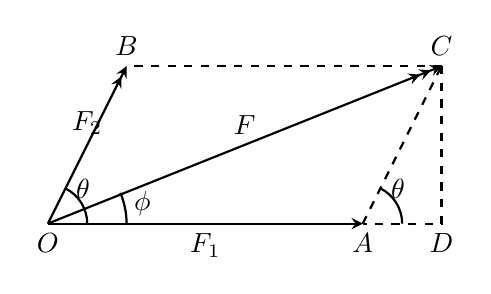
\begin{tikzpicture}[>=stealth,  thick]
\draw [->](0,0)node[below] {$O$}--node[below] {$F_1$} (4,0)node[below] {$A$} ;
\draw [->>](0,0)--node[above] {$F_2$}(1,2) node[above] {$B$};
\draw [dashed](5,2)--(1,2);
\draw [dashed](4,0)--(5,2)node[above] {$C$};
\draw [->>>](0,0)--node[above] {$F$}(5,2) ;
\draw [dashed](5,2)--(5,0) node[below] {$D$}--(4,0);
\draw (.5,0) arc (0:63:.5) node[right] {$\theta$};
\draw (1,0) arc (0:23:1);
\draw (4.5,0) arc (0:63:.5) node[right] {$\theta$};
\node at (1.2,.25) {$\phi$};
\end{tikzpicture}
\caption{}
\end{figure}


    在三角形$OAC$中,根据余弦定理得到
\[\begin{split}
F^2 & = F_1^2+F_2^2-2F_1F_2\cos(180^\circ -\theta)  \\
&= F_1^2+F_2^2+2F_1F_2\cos\theta
\end{split} \]
所以合力的大小
\begin{equation}
F=\sqrt{F_1^2+F_2^2+2F_1F_2\cos\theta}
\end{equation}

    合力的方向可以用合力跟原来任一个力的夹角表示出
来.图中用$F$跟$F_1$的夹角$\phi$来表示,利用直角三角形$ODC$,
可以求出角$\phi$的正切:
\begin{equation}
\tan\phi =\frac{CD}{OD}=\frac{CD}{OA+AD}=\frac{F_2\sin\theta }{F_1+F_2\cos\theta}
\end{equation}




    根据(1.1)(1.2)两式,可以算出两个共点力的合力的大小和
方向,例如在运河两岸拉着一艘货船前进,两条绳对货船的
拉力都是$2\times 10^3$牛,两绳互成$45^\circ$角(图1.25).合力的大
小是:
\[\begin{split}
F&= \sqrt{F_1^2+F_2^2+2F_1F_2\cos\theta}\\
&=\sqrt{(2\times 10^3)^2+(2\times 10^3)^2+2(2\times 10^3)^2\cos 45^{\circ}}\text{牛}\\
&=3.7\times 10^3\text{牛.}
\end{split} \]
\[\begin{split}
\tan\phi&= \frac{F_2\sin\theta }{F_1+F_2\cos\theta}\\
&= \frac{2\times 10^3\times \sin 45^{\circ}}{2\times 10^3+2\times 10^3\times \cos 45^{\circ}}  \\
&=0.4142\\
\phi &= 22^{\circ} 30'
\end{split} \]

\begin{figure}[htp]
\centering
\includegraphics[scale=.5]{fig/1-25.png}
\caption{}
\end{figure}

    由于$F_1=F_2$,利用力的平行四边形,由几何方法容易证
明合力$F$的方向沿着力$F_1$和$F_2$的夹角平分线的方向.这跟
应用公式(1.2)算出夹角$\phi$来表示合力的方向是一致的.

    现在我们来讨论,力$F_1$和$F_2$的大小一定的时候,合力$F$
的大小跟两个力的夹角$\theta$的关系.

\begin{figure}[htp]
\centering
\begin{tikzpicture}[>=stealth,  thick]
\draw [fill=black!20](0,1.5) circle[radius=.3];
\fill (0,1.5) circle[radius=1.5pt];
\draw [->](0,1.5)--(1,1.5) node [above] {$F_1$};
\draw [->](0,1.5)--(2,1.5) node [right] {$F_2$};


\draw [fill=black!20](0,0) circle[radius=.3];
\fill (0,0) circle[radius=1.5pt];
\draw [->](0,0)--(3,0) node [right] {$F$};
\node at (1.5, -.75){甲};
\end{tikzpicture}\qquad 
\begin{tikzpicture}[>=stealth,  thick]
\draw [fill=black!20](0,1.5) circle[radius=.3];
\fill (0,1.5) circle[radius=1.5pt];
\draw [->](0,1.5)--(3,1.5) node [above] {$F_1$};
\draw [->](0,1.5)--(-2,1.5) node [above] {$F_2$};

\node at (.5, -.75){乙};
\draw [fill=black!20](0,0) circle[radius=.3];
\fill (0,0) circle[radius=1.5pt];
\draw [->](0,0)--(1,0) node [right] {$F$};
\end{tikzpicture}
\caption{}
\end{figure}

    当两个力的方向相同时(图1.26甲),$\theta =0^\circ$,$\cos 0^\circ=1$,
所以$F=F_1+F_2$,合力的大小等于两个力的大小之和,合力的
方向跟两个力的方向相同.

    当两个力的方向相反时(图1.26乙),$\theta =180^\circ$,$\cos 180^\circ=-1$,
所以$F=F_1-F_2$,合力的大小等于两个力的大小之差,
方向跟两个力中较大的那几个力的方向相同.如果力$F_1$和$F_2$
的大小相等,合力就等于零.

    当$F_1$和$F_2$的夹角$\theta$在$0^\circ$到$180^\circ$之间时,$\theta$越大,
$\cos\theta$的值越小,合力就越小,而且合力的方向也随着夹角$\theta$的变化
而变化.


\subsection*{练习六}
\begin{enumerate}
\item 两个力的合力总大于原来的每一个力,这话对吗?为
什么?

\item 有两个力$F_1$和$F_2$,用作图法求出当它们之间的夹角
$\theta =0^\circ$, $30^\circ$, $60^\circ$, $90^\circ$, $120^\circ$, $150^\circ$, $180^\circ$时的合力.研究你所作
的图,能不能得到结论:夹角$\theta$在$0^\circ$到$180^\circ$之间时,$\theta $越大,合
力就越小.
\item 两个力的合力什么情况下最大,什么情况下最小?设
有两个力,一个是20牛,一个走5牛.合力的最大值是多大,最
小位是多大?
\item 2牛和10牛的两个力,它们的合力能够等于5牛、10牛、
15牛吗?
\item   两个力互成$30^\circ$角, 大小分别是90牛和120牛.用作图法求出合力的
大小和方向,然后再用公式来求.
\end{enumerate}
    
\section{力的分解}
作用在物体上的一个力往往产生几个效果.拖拉机拉犁
耕地,对犁的拉力$F$是斜向上方的,这个力产生两个效果:使
犁克服泥土的阻力前进,同时把犁上提.这两个效果相当于
两个力产生的(图1.27):一个水平的力$F_1$使犁前进,一个竖
直向上的力$F_2$把犁上提.可见力$F$可以用两个力$F_1$和$F_2$
来代替几个力,如果它们产生的效果跟原来一个力产生的
效果相同,这几个力就叫做原来那个力的\textbf{分力}.求一个已知
力的分力叫做\textbf{力的分解}.

\begin{figure}[htp]\centering
\includegraphics[scale=.5]{fig/1-27.png}
\caption{}
\end{figure}

    因为分力的合力就是原来被分解的那个力,力的分解是
力的合成的逆运算,所以一个力分解为两个力同样遵守平行
四边形法则.把一个已知力作为平行四边形的对角线,那么
与已知力共点的平行四边形的两个邻边就是已知力的两个分
力.在图1.27中,$F_1$和$F_2$是$F$的两个分力.


    我们知道,如果没有其他限制,对于同一条对角线,可以
作出无数个不同的平行四边形(图1.28)也就是说,同一个
力$F$可以分解为无数对大小、方向不同的分力.那么,一个己
知力究竟该怎样分解呢?

    把一个物体放在斜面上,物体受到竖直向下的重力,但
它并不能竖直下落,而要沿着斜面下滑,同时使斜面受到压
力.这时重力产生两个效果:使物体沿斜面下滑以及使物体
压紧斜面.因此重力$G$应该分解为这样两个力:平行于斜面
使物体下滑的力$F_1$,垂直于斜面使物体压紧斜面的力$F_2$(图
1.29).


\begin{figure}[htp]
\centering
\begin{minipage}[t]{0.48\textwidth}
\centering
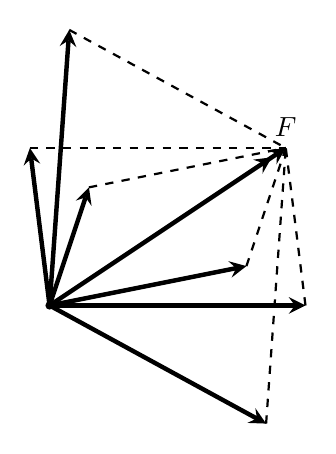
\begin{tikzpicture}[>=stealth,  thick]

\fill (0,0) circle[radius=1.5pt];
\draw [->>, ultra thick](0,0)--(3,2) node [above] {$F$};
\draw [->, ultra thick](0,0)--(.5,1.5) ;
\draw [dashed](.5,1.5)--(3,2) ;
\draw [->, ultra thick](0,0)--(2.5,.5) ;
\draw [dashed](2.5,.5)--(3,2) ;

\draw [->, ultra thick](0,0)--(.25,3.5) ;
\draw [dashed](.25,3.5)--(3,2) ;
\draw [->, ultra thick](0,0)--(2.75,-1.5) ;
\draw [dashed](2.75,-1.5)--(3,2) ;

\draw [->, ultra thick](0,0)--(-.25,2) ;
\draw [dashed](-.25,2)--(3,2) ;
\draw [->, ultra thick](0,0)--(3.25,0) ;
\draw [dashed](3.25,0)--(3,2) ;


\end{tikzpicture}
\caption{}
\end{minipage}
\begin{minipage}[t]{0.48\textwidth}
\centering
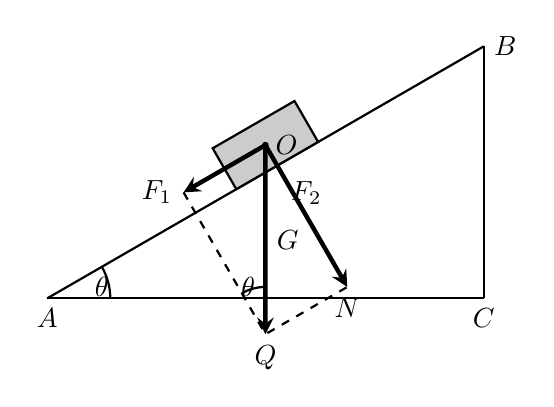
\begin{tikzpicture}[>=stealth,  thick, scale=.8]


\draw (0,0)node[below]{$A$}--(6.93,0) node[below]{$C$};
\draw (6.93,0)--(6.93,4) node[right]{$B$};
\draw (0,0)--(6.93,4);
\draw [rotate=30, fill=black!20] (6.93/2,0) rectangle (6.93/2+1.5,0+.75);

\draw [rotate=30, ->, ultra thick] (6.93/2+.75,.75/2)--node [above]{$F_2$} (6.93/2+.75,.75/2-2.6) node [below]{$N$};
\draw [rotate=30, ->, ultra thick] (6.93/2+.75,.75/2)-- (6.93/2+.75-1.5,.75/2)node [left]{$F_1$};
\draw [rotate=30, ->, ultra thick] (6.93/2+.75,.75/2)--node [right]{$G$} (6.93/2+.75-1.5,.75/2-2.6)node [below]{$Q$};
\draw [rotate=30, dashed] (6.93/2+.75-1.5,.75/2)--(6.93/2+.75-1.5,.75/2-2.6)-- (6.93/2+.75,.75/2-2.6);


\fill [rotate=30] (6.93/2+.75,.75/2) circle[radius=1.5pt] node [right]{$O$};

\draw [rotate=30](6.93/2+.75-1.5,.75/2-2.6+.75) arc(90:60:.75)node [left]{$\theta$};

\draw (0+1, 0) arc(0:30:1)node [below]{$\theta$};

\end{tikzpicture}
\caption{}
\end{minipage}
\end{figure}

    如果已知斜面的倾角$\theta$,就可以求出分力$F_1$和$F_2$的大
小.由于直角三角形$ABC$与$OQN$相似,所以
\[\begin{split}
F_1&= G\sin\theta, \\
F_2&= G\cos\theta. \\
\end{split} \]
可以看出,$F_1$和$F_2$的大小都和斜面的倾角有关.斜面的倾
角增大时,$F_1$增大,$F_2$减小.车辆上桥时,力$F_1$阻碍车辆前
进;车辆下桥时,力$F_1$使车辆运动加快.为了行车方便与安
全,高大的桥要造很长的引桥,来减小桥面的坡度.

    把重量为$G$的物体挂在图1.30所示的支架上,物体通过
绳子使支架上的$O$点受到一个向下的作用力$F$,大小等于物
体的重量$G$.力$F$对支架的两个梁产生的效果是什么呢?如
果在$M$和$N$处加上小弹簧,可以看到$M$处的弹簧受到压缩,$N$
处的弹簧受到拉伸.这时力$F$产生两个效果:沿$NO$方向拉
斜梁,沿$OM$方向压横梁.因
此应该把力$F$分解为这样两个
力:沿$NO$方向拉斜梁的力$F_1$,
沿$OM$方向压横梁的力$F_2$.设
斜梁跟墙的夹角为$\theta$,可以看出,
\[\begin{split}
F_1&= F/\cos\theta, \\
F_2&= F\tan\theta. \\
\end{split} \]

\begin{figure}[htp]
\centering
\begin{minipage}[t]{0.48\textwidth}
\centering
\begin{tikzpicture}[>=stealth,  thick, scale=1.25]

\fill [pattern = north east lines] (-0.25,-2) rectangle (0,2);
\draw (0,-2)--(0,2);

\draw[->, very thick](2.5,0)--(2.5*1.5, -.9)node [right]{$F_1$};

\draw[->, very thick](2.5,0)--(2.5,-.9)node [left]{$F$};

\draw (2.5,0)--(2.5, -1.5);
\draw[dashed](2.5*.5, 0)--(2.5,-.9)--(2.5*1.5, -.9);



\draw[fill=black!40](2,-2) rectangle (3,-1.5);
\draw (0,1.8-.25) arc(270:325:.25) node [below]{$\theta$};
\draw (2.5,0-.25) arc(270:325:.25) node [below]{$\theta$};

\pgfsetlinewidth{2pt}
\pgfsetinnerlinewidth{1pt}
\draw[line width=.5ex] (0,1.8)node [right]{$N$}--(2.5,0)node [right]{$O$};
\draw[line width=.5ex] (0,0)--(2.5,0);
\draw[->](2.5,0)--(2.5*.5, 0)node [above]{$F_2$};
\node at (.2,-.2) {$M$};



\end{tikzpicture}
\caption{}
\end{minipage}
\begin{minipage}[t]{0.48\textwidth}
\centering
\centering\includegraphics[scale=.5]{fig/1-31.png}
\caption{}
\end{minipage}
\end{figure}

    从上述例子可以看出,分解一个力要具体考虑这个力产
生的效果,一个力我们可以根据它产生的效果来分解它.


\subsection*{练习七}
\begin{enumerate}

\item 一个物体的重量是20牛,把它放在一个斜面上,斜面
长$AB$与斜面高$BC$之比是$5:3$.把重力分解,求出平行于斜面
使物体下滑的力和垂直于斜面使物体压紧斜面的力.
 


\item 图1.31是塔式起重机,钢索$NO$与水平悬臂$MO$成
$30^\circ$角,当起重机吊着$4.0\times 10^4$牛的货物时,钢索和悬臂分别受
多大的力?
\item 如图1.32所示,垂直作用在帆上的风力$F=1.0\times 10^4$
牛.沿着船身方向的分力$F_1$使帆船前进,垂直于船身方向的
分力$F_2$使船身侧倾.设$F$与船身方向成$45^\circ$角,求力$F_1$是多大.
\begin{figure}[htp]
\centering\includegraphics[scale=.5]{fig/1-32.png}
\caption{}
\end{figure}

\item 把竖直向下的180牛的力分解为两个分力,一个分力
在水平方向上并等于240牛,求另一个分力的大小和方向.

\item 一个小同学跟一个大同学拔河,小同学拉不动大同
学,可是用下述办法,小同学就可以拉动大同学.在树干上
拴一条绳子,大同学拿着绳子的另一端,沿水平方向把绳子拉
紧.小同学用力推绳子的中点,就可以拉动大同学了.实际
做一做,并解释所发生的现象.

\end{enumerate}

\section{矢量和标量}
    我们在初中学过长度、质量、时间等等物理量.这些物理
量的大小可以用一个带有单位的数值来表示.例如说铅笔长
15厘米,钢块的质量是50千克等等.我们用15厘米就能完
全描述这支铅笔的长度,用50千克就能完全描述这块钢的质
量.力是有大小的,我们也可以用带有单位的数值来表示力.
例如说这个力是10牛,那个力是6牛.可是,这样并没有把
一个力完全表达出来.因为力不但有大小,而且有方向.相
同大小的力,方向不同,它们的作用效果并不相同.要把一个
力完全表达出来,除了说明它的大小,还要指明它的方向才
行.

    这种既有大小又有方向的物理量,除了力而外,在物理学
中还有很多.我们在初中学过的速度也是这类物理量.我们说
一辆汽车的速度是60千米/小时,这并没有把汽车的运动情况完全表达出来,因为这只能说明汽车运动得多快,而没有
说明汽车运动的方向.速度不但有大小,而且有方向.速度
的方向就是物体运动的方向.

    这样,我们就接触到一类物理量.它们的共同特点是:既
有大小,又有方向.这种既有大小又有方向的物理量,叫做\textbf{矢
量}.力是矢量,速度也是矢量.那些只有大小没有方向的物
理量,叫做\textbf{标量}.长度、质量、时间是标量,初中学过的功、温
度等也是标量.

    矢量可以用一根带箭头的线段来表示.线段按一定标度
画出,线段的长短表示矢量的大小,箭头的指向表示矢量的方
向.前面讲的力的图示,其实就是力矢量的表示.速度矢量
以及所有其他矢量都可以这样来表示.

    标量和矢量不仅含义不同,而且服从不同的运算规则.

    两个同类的标量,例如两个质量,只要它们的数值和单位
都相同,比如说都是12千克,我们就说这两个量是相等的.矢
量则不然.两个同类的矢量,它们的大小相等,但方向不同,
就不能说这两个矢量是相等的.比如两个力都是15牛,但方
向不同,就不能说这两个力矢量相等.两个矢量只有大小相
等而且方向相同,才是相等的.

    两个同类的标量,只要单位相同,它们的数值就可以用化
数加法来运算.比如一个质量是10千克,另一个质量是5千
克,总质量就是15千克.矢量则不能这样运算.一个物体受
到两个力,一个是10牛,一个是5牛.这两个力共同作用所
产生的效果不仅决定于它们的大小,而且决定于它们的方向.
前面讲的力的合成就充分说明了这一点.力的合成要按照平
行四边形法则来进行.平行四边形法则不仅适用于力的合
成,对于别的矢量(如速度矢量)同样适用,是矢量合成即矢量
加法运算的普遍法则.

    认识到矢量和标量的不同,这是物理学研究中的一大进
步.有了矢量的概念并且运用矢量的运算规则,我们就能很
方便地研究和处理一些物理问题.

\section{同一直线上的矢量的运算}
    本书中常常要处理同一直线上的矢量,这一节我们以力
矢量为例讲一讲同一直线上的矢量的运算,以备以后的应用.
这里虽然是以力矢量为例来讲的,但对任何矢量都适用.

    矢量既有大小,又有方向.如果被运算的矢量在一条直
线上,那么,我们就可以用一个带有正负号的数值把矢量的大
小和方向都表示出来.为此,我们沿着矢量所在的直线选定
一个正方向(图1.33)规定凡是方向跟正方向相同的矢量都
取正值,凡是方向跟正方向相反的矢量都取负值,例如图中
$F_1=5$牛,$F_2=-5$牛,$F_3=7$牛,$F_4=-5$牛.这里,根据数值
的正负号就可以知道力的方向;而力的大小等于它们的绝对
值,分别是5牛,5牛,7牛,5牛.

\begin{figure}[htp]
\centering
\begin{tikzpicture}[>=stealth,  thick, scale=0.9]

\draw[dashed, ->](0,0)--(13,0) ;
\node at (13,-.5){选定的正方向};
\fill (3,0) circle[radius=2.5pt];
\draw[very thick, ->](3,0)--node[above]{$F_4=-5$牛}(1,0);

\fill (3.5,0) circle[radius=2.5pt];
\draw[very thick, ->](3.5,0)--node[above]{$F_3=7$牛}(6.3,0);

\fill (9,0) circle[radius=2.5pt];
\draw[very thick, ->](9,0)--node[above]{$F_2=-5$牛}(7,0);

\fill (10,0) circle[radius=2.5pt];
\draw[very thick, ->](10,0)--node[above]{$F_1=5$牛}(12,0);
\end{tikzpicture}
\caption{}
\end{figure}

既然同一条直线上的矢量可以用带正负号的数值来表
示,它们的运算就可以简化为代数运算.

    如果两个矢量大小相等而且方向相同,如图1.33中的
$F_2$和$F_4$,我们就说这两个矢量相等,写成代数式就是
\begin{equation}
F_2-F_4
\end{equation}

    如果两个矢量大小相等而方向相反,如图1.33中的$F_1$和$F_2$,
那么,它们只是符号相反,写成代数式就是
\begin{equation}
F_1=-F_2
\end{equation}

    如图1.34所示,设有两个力$F_1$和$F_2$作用在一个物体
上,我们可以利用加法运算求出合力$F$:
\begin{equation}
\begin{split}
F&=F_1+F_2\\
&=10+(-6)=4\text{牛}
\end{split}
\end{equation}
这表示合力的大小是4牛,结果是正值表示合力的方向与选
定的正方向相同,即合力的方向跟两个力中较大的那个力的
方向相同.

\begin{figure}[htp]
\centering
\begin{tikzpicture}[>=stealth,  thick, scale=.7]

\draw[dashed, ->](1,0)--(12,0) node[below]{选定的正方向};

\fill (5,0) circle[radius=2.5pt];
\draw[very thick, ->](5,0)--node[above]{$F_2=-6$牛}(2,0);

\fill (5,0) circle[radius=2.5pt];
\draw[very thick, ->](5,0)--node[above]{$F_1=10$牛}(10,0);
\fill (5,-.75) circle[radius=2.5pt];
\draw[very thick, ->](5,-.75)--node[below]{$F=4$牛}(7,-.75);


\end{tikzpicture}
\caption{}
\end{figure}

    我们也可以利用减法运算求分力.如图1.35所示,已知
合力$F$和一个分力$F_1$,那么,另一个分力$F_2$:
\begin{equation}
\begin{split}
F_2&=F-F_1\\
&=8-(-3)=11\text{牛}
\end{split}
\end{equation}
这表示$F_2$的大小是11牛,方向与选定的正方向相同.

需要强调指出的是:\textit{只有同一直线上的矢量,它们的运
算才可以象上述那样简化成代数运算.这是平行四边形法则
在这种特殊情况下的运用}.不在同一直线上的矢量,它们的运算不能
这样简化成代数运算,仍必须按照平行四边形法则
来进行.

\begin{figure}[htp]
\centering
\begin{tikzpicture}[>=stealth,  thick, scale=.7]

\draw[dashed, ->](2,0)--(11,0) node[right]{选定的正方向};

\fill (5,0) circle[radius=2.5pt];
\draw[very thick, ->](5,0)--node[above]{$F_1=-3$牛}(3.5,0);

\fill (5,0) circle[radius=2.5pt];
\draw[very thick, ->](5,0)--node[above]{$F=8$牛}(9,0);
\fill (5,-.5) circle[radius=2.5pt];
\draw[very thick, ->](5,-.5)--node[below]{$F_2=11$牛}(10.5,-.5);


\end{tikzpicture}
\caption{}
\end{figure}

    还要指出的是:这里用带有正负号的数值既表示出矢量
的大小,又表示出矢量的方向;如果专指矢量的大小,就要取
绝对值,即矢量的大小总是正值.本章前面各节中的公式,如
公式
\[\begin{split}
f&=kx\\
f&=\mu N\\
F&=\sqrt{F^2_1+F^2_2+2F_1F_2\cos\theta}\\
F&=F_1+F_2\quad (\theta =0^\circ)\\
F&=F_1-F_2\quad (\theta =180^\circ)\\
\end{split} \]
等等都是关于力矢量大小的公式.利用这些公式来计算.其
中的各力都取正值.例如用$F=F_1-F_2$来计算图1.34中的
合力时,$F_1=10$牛,$F_2=5$牛,$F=F_1-F_2=4$牛.这与
(1.5)式
所得结果相同.初学时概念上要弄清楚,熟悉起来以后,就可
以根据物理思考灵活运用了.


\subsection*{复习题}

\begin{enumerate}
\item 从力的性质看,力学中经常遇到的有哪几种力?这几
种力的情况是怎样的?力可以用哪两种方法来分类?为什么说
拉力、压力和支持力都是弹力?
\item
胡克定律的内容是什么?写出胡克定律的公式.
\item
怎样计算滑动摩擦力的大小?写出它的公式.
\item 牛顿第三定律的内容是什么,为什么说作用力和反
作用力不能互相平衡?
\item
力的合成要按照什么法则来进行?这个法则的内容
又什么,写出计算合力的大小和方向的公式.
\item
为什么力的分解和合成遵守相同的法则?一个力可
以根据什么来分解它?一个力,如果知道它的两个分力的方
向,或者知道它的一个分力的大小和方向,那么,这个力的分
解有没有确定的答案?
\item
什么叫矢量?什么叫标量?矢量和标量有什么不同?
矢量加法要按照什么法则来运算?
\item
你自己总结一下应该怎样分拆物体的受力情况,分
析时应该注意什么?
\end{enumerate}

\section*{习题}

\begin{enumerate}
\item   如图1.36所示,为了防止电线杆倾倒,常在两侧对称
地拉上钢绳.如果两条钢绳间的夹角是$60^\circ$,每条钢绳的拉力
都是300牛,求两条钢绳作用在电线杆上的合力.

\begin{figure}[htp]
\centering
\begin{minipage}[t]{0.48\textwidth}
\centering
\begin{tikzpicture}[>=stealth,  thick, scale=.7]

\fill [pattern = north east lines] (-3,-.5) rectangle (3,0);
\draw(-3,0)--(3,0);


\draw (0,4.5)--(-2.5,0);
\draw (0,4.5)--(2.5,0);
\foreach \x in{1,2,3}
{
    \draw [fill=white] (-.5,4.8+\x*0.2) rectangle (.5,4.8+\x*0.2+.1);
}
\draw [fill=white] (-.1,0) rectangle (.1,6);


\draw [->](-1.4,3)--(-2,2);
\draw [->](1.4,3)--(2,2);
\end{tikzpicture}
\caption{}
\end{minipage}
\begin{minipage}[t]{0.48\textwidth}
\centering
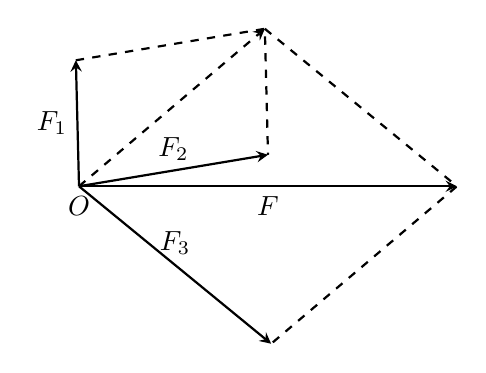
\begin{tikzpicture}[>=stealth,  thick, scale=.8]

\draw [->] (0,0)node [below]{$O$}--node [below]{$F$}(6,0);
\draw [->] (0,0)--node [left]{$F_1$}(-.05, 2);
\draw [->] (0,0)--node [above]{$F_2$}(3, .5);
\draw [dashed] (-.05, 2)--(-.05+3, 2.5)--(3, .5);
\draw [dashed] (-.05+3, 2.5)--(6,0)--(6-3+.05, -2.5);
\draw [->,dashed] (0,0)--(-.05+3, 2.5);
\draw [->] (0,0)--node [above]{$F_3$} (6-3+.05, -2.5);
\end{tikzpicture}
\caption{}
\end{minipage}
\end{figure}


\item  图1.37表示用平行四边形法则求三个共点力$F_1$、$F_2$、$F_3$
的合力$F$.先求出$F_1$和$F_2$的合力,再求出这个合力与$F_3$的
合力$F$.改用三角形法求出这三个力的合力.改变求和的顺
序,再分别用平行四边形法则和三角形法求出这三个力的合
力.



\item   20牛、30牛和40牛的三个力作用于物体的一点,它们
之间的夹角都是$120^\circ$.求合力的大小和方向.

\item 如图1.38所示,把一个重量为10牛的物体挂在绳子
上,已知$AC=BC=3$米,$CD=1$米.求绳$AC$和$BC$所受的拉
力.
\begin{figure}[htp]
\centering
\begin{tikzpicture}[>=stealth,  thick ]

\fill [pattern = north east lines] (-4,-.5) rectangle (-3.8,.5);
\draw(-3.8,.5)--(-3.8,-.5);
\fill [pattern = north east lines] (4,-.5) rectangle (3.8,.5);
\draw(3.8,.5)--(3.8,-.5);

\draw [dashed] (-3.8,0)  --node[above]{$D$} (3.8,0);
\node at (-3.5,0) [below]{$A$};
\node at (3.5,0) [below]{$B$};
\draw [dashed] (0,0)  -- (0,-1.5)node[above]{$C$};
\draw  (0,-1.5)  -- (0,-2.5);
\draw (-3.8,0)--(0,-1.5)--(3.8,0);
\draw [fill=black!30] (-.5,-2.5) rectangle (.5,-2.75-.6);


\end{tikzpicture}
\caption{}
\end{figure}


\item   用手握着橡皮绳的两端,在橡皮绳的中间挂一个重
物,当两手之间的距离增大或减小的时候,物体对橡皮绳的
拉力是否改变?怎样改变?实际做一下,并说明道理.

\item  刀、斧、凿、刨等切削工具的刃部叫做劈,劈的纵截面
是一个三角形,如图1.39所示.使用劈的时候,在劈背上加力
$F$,这个力产生两个效果,这就是使劈的两个侧面推压物体,
把物体劈开.设劈的纵截面是一个等腰三角形,劈背的宽度
是$d$,劈的侧面的长度是$\ell$,可以证明:
\[f_1=f_2=\frac{\ell}{d}F \]

从上式可知,当$F$一定的时侯,劈的两个侧面之间的夹角
越小,$\ell/d$就越大,$f_1$和$f_2$就越大.这说明了为什么越锋利的
切削工具越容易劈开物体.试证明上式.



\item 一个物体放在倾角为$\theta$的光滑斜面上,求物体受到
的合力.
\begin{figure}[htp]\centering
\begin{minipage}[t]{0.48\textwidth}
\centering
\includegraphics[scale=.4]{fig/1-39.png}
\caption{}
\end{minipage}
\begin{minipage}[t]{0.48\textwidth}
\centering
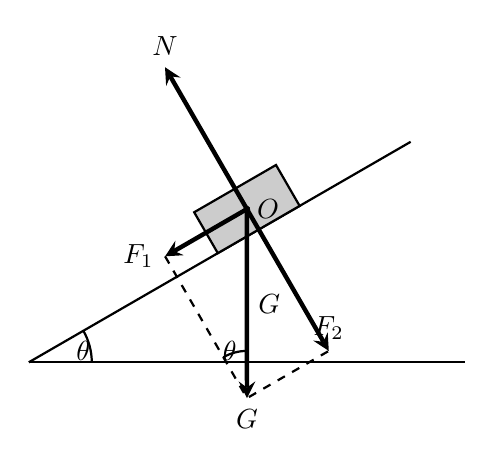
\begin{tikzpicture}[>=stealth,  thick, scale=.8]
\draw (0,0) --(6.93,0) ;
\draw (0,0)--(30:7);
\draw [rotate=30, fill=black!20] (6.93/2,0) rectangle (6.93/2+1.5,0+.75);
\draw [rotate=30, ->, ultra thick] (6.93/2+.75,.75/2)-- (6.93/2+.75,.75/2-2.6) node [above]{$F_2$};
\draw [rotate=30, ->, ultra thick] (6.93/2+.75,.75/2)-- (6.93/2+.75,.75/2+2.6) node [above]{$N$};
\draw [rotate=30, ->, ultra thick] (6.93/2+.75,.75/2)-- (6.93/2+.75-1.5,.75/2)node [left]{$F_1$};
\draw [rotate=30, ->, ultra thick] (6.93/2+.75,.75/2)--node [right]{$G$} (6.93/2+.75-1.5,.75/2-2.6)node [below]{$G$};
\draw [rotate=30, dashed] (6.93/2+.75-1.5,.75/2)--(6.93/2+.75-1.5,.75/2-2.6)-- (6.93/2+.75,.75/2-2.6);
\fill [rotate=30] (6.93/2+.75,.75/2) circle[radius=1.5pt] node [right]{$O$};

\draw [rotate=30](6.93/2+.75-1.5,.75/2-2.6+.75) arc(90:60:.75)node [left]{$\theta$};

\draw (0+1, 0) arc(0:30:1)node [below]{$\theta$};

\end{tikzpicture}
\caption{}
\end{minipage}
\end{figure}

\begin{solution}
放在斜面上的物体受到两个力的作用:重力$G$和斜
面的支持力$N$(图1.40),现在已知$N$的方向,但不知道$N$的
大小.我们把重力$G$分解为两个分力:平行于斜面的分力
$F_1=G\sin\theta$,垂直于斜面的分力$F_2=G\cos\theta$.这样,物体相当
于受到$G\sin\theta$、$G\cos\theta$和$N$这三个力的作用.因为物体沿着斜
面运动,在垂直于斜面的方向上不发生运动,所以垂直于斜面
方向的两个力$N$和$G\cos\theta$是互相平衡的,它们大小相等,即
$N=G\cos\theta$.因此,物体受到的合力的大小为$G\sin\theta$,方向平行
于斜面向下.


 \hskip 2em    这里我们先把一个力分解,然后求出合力.这种方法以
后我们还会用到.

 \hskip 2em    我们看到,放在光滑斜面上的物体,所受的合力实际上等
于重力的一个分力$G\sin\theta$,在这个力的作用下物体将沿着斜
面下滑,但是,如果斜面不是光滑的,或者物体还受到别的力,
合力将不再等于重力的一个分力$G\sin\theta$.
\end{solution}
   

\item 一个滑雪人沿着山坡滑下.滑雪人的重量是700牛,
山坡的倾角是$30^\circ$,滑雪板和雪地的滑动摩擦系数是0.04.求
滑雪人所受的合力.

\end{enumerate}


















